% Graphic for TeX using PGF
% Title: /home/ondra/thesis/text/images/pykaldi-classes.dia
% Creator: Dia v0.97.2
% CreationDate: Thu Aug  1 09:11:20 2013
% For: ondra
% \usepackage{tikz}
% The following commands are not supported in PSTricks at present
% We define them conditionally, so when they are implemented,
% this pgf file will use them.
\ifx\du\undefined
  \newlength{\du}
\fi
\setlength{\du}{15\unitlength}
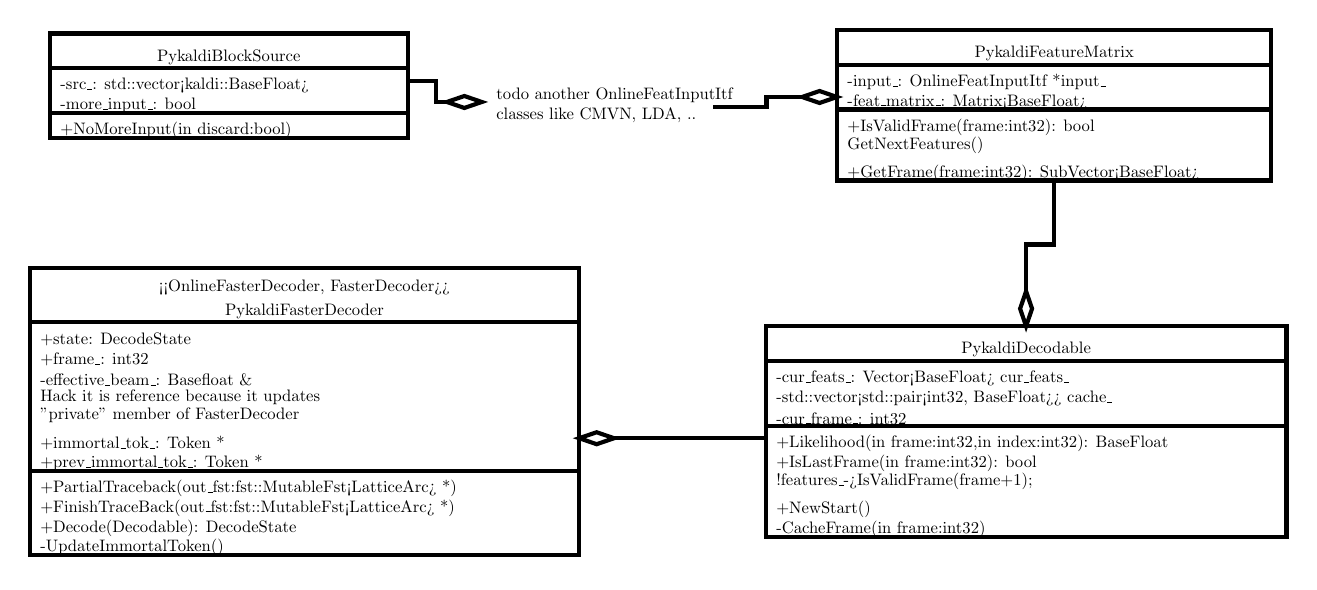
\begin{tikzpicture}[thick,scale=0.6, every node/.style={scale=0.6}]
% \begin{tikzpicture}
\pgftransformxscale{1.000000}
\pgftransformyscale{-1.000000}
\definecolor{dialinecolor}{rgb}{0.000000, 0.000000, 0.000000}
\pgfsetstrokecolor{dialinecolor}
\definecolor{dialinecolor}{rgb}{1.000000, 1.000000, 1.000000}
\pgfsetfillcolor{dialinecolor}
\pgfsetlinewidth{0.100000\du}
\pgfsetdash{}{0pt}
\definecolor{dialinecolor}{rgb}{1.000000, 1.000000, 1.000000}
\pgfsetfillcolor{dialinecolor}
\fill (-24.429682\du,2.054240\du)--(-24.429682\du,3.454240\du)--(-10.069682\du,3.454240\du)--(-10.069682\du,2.054240\du)--cycle;
\definecolor{dialinecolor}{rgb}{0.000000, 0.000000, 0.000000}
\pgfsetstrokecolor{dialinecolor}
\draw (-24.429682\du,2.054240\du)--(-24.429682\du,3.454240\du)--(-10.069682\du,3.454240\du)--(-10.069682\du,2.054240\du)--cycle;
% setfont left to latex
\definecolor{dialinecolor}{rgb}{0.000000, 0.000000, 0.000000}
\pgfsetstrokecolor{dialinecolor}
\node at (-17.249682\du,3.004240\du){PykaldiBlockSource};
\definecolor{dialinecolor}{rgb}{1.000000, 1.000000, 1.000000}
\pgfsetfillcolor{dialinecolor}
\fill (-24.429682\du,3.454240\du)--(-24.429682\du,5.254240\du)--(-10.069682\du,5.254240\du)--(-10.069682\du,3.454240\du)--cycle;
\definecolor{dialinecolor}{rgb}{0.000000, 0.000000, 0.000000}
\pgfsetstrokecolor{dialinecolor}
\draw (-24.429682\du,3.454240\du)--(-24.429682\du,5.254240\du)--(-10.069682\du,5.254240\du)--(-10.069682\du,3.454240\du)--cycle;
% setfont left to latex
\definecolor{dialinecolor}{rgb}{0.000000, 0.000000, 0.000000}
\pgfsetstrokecolor{dialinecolor}
\node[anchor=west] at (-24.279682\du,4.154240\du){-src\_: std::vector<kaldi::BaseFloat>};
% setfont left to latex
\definecolor{dialinecolor}{rgb}{0.000000, 0.000000, 0.000000}
\pgfsetstrokecolor{dialinecolor}
\node[anchor=west] at (-24.279682\du,4.954240\du){-more\_input\_: bool};
\definecolor{dialinecolor}{rgb}{1.000000, 1.000000, 1.000000}
\pgfsetfillcolor{dialinecolor}
\fill (-24.429682\du,5.254240\du)--(-24.429682\du,6.254240\du)--(-10.069682\du,6.254240\du)--(-10.069682\du,5.254240\du)--cycle;
\definecolor{dialinecolor}{rgb}{0.000000, 0.000000, 0.000000}
\pgfsetstrokecolor{dialinecolor}
\draw (-24.429682\du,5.254240\du)--(-24.429682\du,6.254240\du)--(-10.069682\du,6.254240\du)--(-10.069682\du,5.254240\du)--cycle;
% setfont left to latex
\definecolor{dialinecolor}{rgb}{0.000000, 0.000000, 0.000000}
\pgfsetstrokecolor{dialinecolor}
\node[anchor=west] at (-24.279682\du,5.954240\du){+NoMoreInput(in discard:bool)};
\pgfsetlinewidth{0.100000\du}
\pgfsetdash{}{0pt}
\definecolor{dialinecolor}{rgb}{1.000000, 1.000000, 1.000000}
\pgfsetfillcolor{dialinecolor}
\fill (7.170318\du,1.904240\du)--(7.170318\du,3.304240\du)--(24.610318\du,3.304240\du)--(24.610318\du,1.904240\du)--cycle;
\definecolor{dialinecolor}{rgb}{0.000000, 0.000000, 0.000000}
\pgfsetstrokecolor{dialinecolor}
\draw (7.170318\du,1.904240\du)--(7.170318\du,3.304240\du)--(24.610318\du,3.304240\du)--(24.610318\du,1.904240\du)--cycle;
% setfont left to latex
\definecolor{dialinecolor}{rgb}{0.000000, 0.000000, 0.000000}
\pgfsetstrokecolor{dialinecolor}
\node at (15.890318\du,2.854240\du){PykaldiFeatureMatrix};
\definecolor{dialinecolor}{rgb}{1.000000, 1.000000, 1.000000}
\pgfsetfillcolor{dialinecolor}
\fill (7.170318\du,3.304240\du)--(7.170318\du,5.104240\du)--(24.610318\du,5.104240\du)--(24.610318\du,3.304240\du)--cycle;
\definecolor{dialinecolor}{rgb}{0.000000, 0.000000, 0.000000}
\pgfsetstrokecolor{dialinecolor}
\draw (7.170318\du,3.304240\du)--(7.170318\du,5.104240\du)--(24.610318\du,5.104240\du)--(24.610318\du,3.304240\du)--cycle;
% setfont left to latex
\definecolor{dialinecolor}{rgb}{0.000000, 0.000000, 0.000000}
\pgfsetstrokecolor{dialinecolor}
\node[anchor=west] at (7.320318\du,4.004240\du){-input\_: OnlineFeatInputItf *input\_};
% setfont left to latex
\definecolor{dialinecolor}{rgb}{0.000000, 0.000000, 0.000000}
\pgfsetstrokecolor{dialinecolor}
\node[anchor=west] at (7.320318\du,4.804240\du){-feat\_matrix\_: Matrix<BaseFloat>};
\definecolor{dialinecolor}{rgb}{1.000000, 1.000000, 1.000000}
\pgfsetfillcolor{dialinecolor}
\fill (7.170318\du,5.104240\du)--(7.170318\du,7.954240\du)--(24.610318\du,7.954240\du)--(24.610318\du,5.104240\du)--cycle;
\definecolor{dialinecolor}{rgb}{0.000000, 0.000000, 0.000000}
\pgfsetstrokecolor{dialinecolor}
\draw (7.170318\du,5.104240\du)--(7.170318\du,7.954240\du)--(24.610318\du,7.954240\du)--(24.610318\du,5.104240\du)--cycle;
% setfont left to latex
\definecolor{dialinecolor}{rgb}{0.000000, 0.000000, 0.000000}
\pgfsetstrokecolor{dialinecolor}
\node[anchor=west] at (7.320318\du,5.804240\du){+IsValidFrame(frame:int32): bool};
% setfont left to latex
\definecolor{dialinecolor}{rgb}{0.000000, 0.000000, 0.000000}
\pgfsetstrokecolor{dialinecolor}
\node[anchor=west] at (7.320318\du,6.529240\du){GetNextFeatures()};
% setfont left to latex
\definecolor{dialinecolor}{rgb}{0.000000, 0.000000, 0.000000}
\pgfsetstrokecolor{dialinecolor}
\node[anchor=west] at (7.320318\du,7.654240\du){+GetFrame(frame:int32): SubVector<BaseFloat>};
% setfont left to latex
\definecolor{dialinecolor}{rgb}{0.000000, 0.000000, 0.000000}
\pgfsetstrokecolor{dialinecolor}
\node[anchor=west] at (-6.779682\du,4.554240\du){todo another OnlineFeatInputItf};
% setfont left to latex
\definecolor{dialinecolor}{rgb}{0.000000, 0.000000, 0.000000}
\pgfsetstrokecolor{dialinecolor}
\node[anchor=west] at (-6.779682\du,5.354240\du){classes like CMVN, LDA, ..};
\pgfsetlinewidth{0.100000\du}
\pgfsetdash{}{0pt}
\definecolor{dialinecolor}{rgb}{1.000000, 1.000000, 1.000000}
\pgfsetfillcolor{dialinecolor}
\fill (4.310418\du,13.804250\du)--(4.310418\du,15.204250\du)--(25.215418\du,15.204250\du)--(25.215418\du,13.804250\du)--cycle;
\definecolor{dialinecolor}{rgb}{0.000000, 0.000000, 0.000000}
\pgfsetstrokecolor{dialinecolor}
\draw (4.310418\du,13.804250\du)--(4.310418\du,15.204250\du)--(25.215418\du,15.204250\du)--(25.215418\du,13.804250\du)--cycle;
% setfont left to latex
\definecolor{dialinecolor}{rgb}{0.000000, 0.000000, 0.000000}
\pgfsetstrokecolor{dialinecolor}
\node at (14.762918\du,14.754250\du){PykaldiDecodable};
\definecolor{dialinecolor}{rgb}{1.000000, 1.000000, 1.000000}
\pgfsetfillcolor{dialinecolor}
\fill (4.310418\du,15.204250\du)--(4.310418\du,17.804250\du)--(25.215418\du,17.804250\du)--(25.215418\du,15.204250\du)--cycle;
\definecolor{dialinecolor}{rgb}{0.000000, 0.000000, 0.000000}
\pgfsetstrokecolor{dialinecolor}
\draw (4.310418\du,15.204250\du)--(4.310418\du,17.804250\du)--(25.215418\du,17.804250\du)--(25.215418\du,15.204250\du)--cycle;
% setfont left to latex
\definecolor{dialinecolor}{rgb}{0.000000, 0.000000, 0.000000}
\pgfsetstrokecolor{dialinecolor}
\node[anchor=west] at (4.460418\du,15.904250\du){-cur\_feats\_: Vector<BaseFloat> cur\_feats\_};
% setfont left to latex
\definecolor{dialinecolor}{rgb}{0.000000, 0.000000, 0.000000}
\pgfsetstrokecolor{dialinecolor}
\node[anchor=west] at (4.460418\du,16.704250\du){-std::vector<std::pair<int32, BaseFloat>> cache\_};
% setfont left to latex
\definecolor{dialinecolor}{rgb}{0.000000, 0.000000, 0.000000}
\pgfsetstrokecolor{dialinecolor}
\node[anchor=west] at (4.460418\du,17.504250\du){-cur\_frame\_: int32};
\definecolor{dialinecolor}{rgb}{1.000000, 1.000000, 1.000000}
\pgfsetfillcolor{dialinecolor}
\fill (4.310418\du,17.804250\du)--(4.310418\du,22.254250\du)--(25.215418\du,22.254250\du)--(25.215418\du,17.804250\du)--cycle;
\definecolor{dialinecolor}{rgb}{0.000000, 0.000000, 0.000000}
\pgfsetstrokecolor{dialinecolor}
\draw (4.310418\du,17.804250\du)--(4.310418\du,22.254250\du)--(25.215418\du,22.254250\du)--(25.215418\du,17.804250\du)--cycle;
% setfont left to latex
\definecolor{dialinecolor}{rgb}{0.000000, 0.000000, 0.000000}
\pgfsetstrokecolor{dialinecolor}
\node[anchor=west] at (4.460418\du,18.504250\du){+Likelihood(in frame:int32,in index:int32): BaseFloat};
% setfont left to latex
\definecolor{dialinecolor}{rgb}{0.000000, 0.000000, 0.000000}
\pgfsetstrokecolor{dialinecolor}
\node[anchor=west] at (4.460418\du,19.304250\du){+IsLastFrame(in frame:int32): bool};
% setfont left to latex
\definecolor{dialinecolor}{rgb}{0.000000, 0.000000, 0.000000}
\pgfsetstrokecolor{dialinecolor}
\node[anchor=west] at (4.460418\du,20.029250\du){!features\_->IsValidFrame(frame+1);};
% setfont left to latex
\definecolor{dialinecolor}{rgb}{0.000000, 0.000000, 0.000000}
\pgfsetstrokecolor{dialinecolor}
\node[anchor=west] at (4.460418\du,21.154250\du){+NewStart()};
% setfont left to latex
\definecolor{dialinecolor}{rgb}{0.000000, 0.000000, 0.000000}
\pgfsetstrokecolor{dialinecolor}
\node[anchor=west] at (4.460418\du,21.954250\du){-CacheFrame(in frame:int32)};
\pgfsetlinewidth{0.100000\du}
\pgfsetdash{}{0pt}
\definecolor{dialinecolor}{rgb}{1.000000, 1.000000, 1.000000}
\pgfsetfillcolor{dialinecolor}
\fill (-25.239582\du,11.454250\du)--(-25.239582\du,13.654250\du)--(-3.179582\du,13.654250\du)--(-3.179582\du,11.454250\du)--cycle;
\definecolor{dialinecolor}{rgb}{0.000000, 0.000000, 0.000000}
\pgfsetstrokecolor{dialinecolor}
\draw (-25.239582\du,11.454250\du)--(-25.239582\du,13.654250\du)--(-3.179582\du,13.654250\du)--(-3.179582\du,11.454250\du)--cycle;
% setfont left to latex
\definecolor{dialinecolor}{rgb}{0.000000, 0.000000, 0.000000}
\pgfsetstrokecolor{dialinecolor}
\node at (-14.209582\du,12.254250\du){<<OnlineFasterDecoder, FasterDecoder>>};
% setfont left to latex
\definecolor{dialinecolor}{rgb}{0.000000, 0.000000, 0.000000}
\pgfsetstrokecolor{dialinecolor}
\node at (-14.209582\du,13.204250\du){PykaldiFasterDecoder};
\definecolor{dialinecolor}{rgb}{1.000000, 1.000000, 1.000000}
\pgfsetfillcolor{dialinecolor}
\fill (-25.239582\du,13.654250\du)--(-25.239582\du,19.604250\du)--(-3.179582\du,19.604250\du)--(-3.179582\du,13.654250\du)--cycle;
\definecolor{dialinecolor}{rgb}{0.000000, 0.000000, 0.000000}
\pgfsetstrokecolor{dialinecolor}
\draw (-25.239582\du,13.654250\du)--(-25.239582\du,19.604250\du)--(-3.179582\du,19.604250\du)--(-3.179582\du,13.654250\du)--cycle;
% setfont left to latex
\definecolor{dialinecolor}{rgb}{0.000000, 0.000000, 0.000000}
\pgfsetstrokecolor{dialinecolor}
\node[anchor=west] at (-25.089582\du,14.354250\du){+state: DecodeState};
% setfont left to latex
\definecolor{dialinecolor}{rgb}{0.000000, 0.000000, 0.000000}
\pgfsetstrokecolor{dialinecolor}
\node[anchor=west] at (-25.089582\du,15.154250\du){+frame\_: int32};
% setfont left to latex
\definecolor{dialinecolor}{rgb}{0.000000, 0.000000, 0.000000}
\pgfsetstrokecolor{dialinecolor}
\node[anchor=west] at (-25.089582\du,15.954250\du){-effective\_beam\_: Basefloat \&};
% setfont left to latex
\definecolor{dialinecolor}{rgb}{0.000000, 0.000000, 0.000000}
\pgfsetstrokecolor{dialinecolor}
\node[anchor=west] at (-25.089582\du,16.679250\du){Hack it is reference because it updates};
\definecolor{dialinecolor}{rgb}{0.000000, 0.000000, 0.000000}
\pgfsetstrokecolor{dialinecolor}
\node[anchor=west] at (-25.089582\du,17.379250\du){"private" member of FasterDecoder};
% setfont left to latex
\definecolor{dialinecolor}{rgb}{0.000000, 0.000000, 0.000000}
\pgfsetstrokecolor{dialinecolor}
\node[anchor=west] at (-25.089582\du,18.504250\du){+immortal\_tok\_: Token *};
% setfont left to latex
\definecolor{dialinecolor}{rgb}{0.000000, 0.000000, 0.000000}
\pgfsetstrokecolor{dialinecolor}
\node[anchor=west] at (-25.089582\du,19.304250\du){+prev\_immortal\_tok\_: Token *};
\definecolor{dialinecolor}{rgb}{1.000000, 1.000000, 1.000000}
\pgfsetfillcolor{dialinecolor}
\fill (-25.239582\du,19.604250\du)--(-25.239582\du,23.004250\du)--(-3.179582\du,23.004250\du)--(-3.179582\du,19.604250\du)--cycle;
\definecolor{dialinecolor}{rgb}{0.000000, 0.000000, 0.000000}
\pgfsetstrokecolor{dialinecolor}
\draw (-25.239582\du,19.604250\du)--(-25.239582\du,23.004250\du)--(-3.179582\du,23.004250\du)--(-3.179582\du,19.604250\du)--cycle;
% setfont left to latex
\definecolor{dialinecolor}{rgb}{0.000000, 0.000000, 0.000000}
\pgfsetstrokecolor{dialinecolor}
\node[anchor=west] at (-25.089582\du,20.304250\du){+PartialTraceback(out\_fst:fst::MutableFst<LatticeArc> *)};
% setfont left to latex
\definecolor{dialinecolor}{rgb}{0.000000, 0.000000, 0.000000}
\pgfsetstrokecolor{dialinecolor}
\node[anchor=west] at (-25.089582\du,21.104250\du){+FinishTraceBack(out\_fst:fst::MutableFst<LatticeArc> *)};
% setfont left to latex
\definecolor{dialinecolor}{rgb}{0.000000, 0.000000, 0.000000}
\pgfsetstrokecolor{dialinecolor}
\node[anchor=west] at (-25.089582\du,21.904250\du){+Decode(Decodable): DecodeState};
% setfont left to latex
\definecolor{dialinecolor}{rgb}{0.000000, 0.000000, 0.000000}
\pgfsetstrokecolor{dialinecolor}
\node[anchor=west] at (-25.089582\du,22.704250\du){-UpdateImmortalToken()};
\pgfsetlinewidth{0.100000\du}
\pgfsetdash{}{0pt}
\pgfsetmiterjoin
\pgfsetbuttcap
{
\definecolor{dialinecolor}{rgb}{0.000000, 0.000000, 0.000000}
\pgfsetfillcolor{dialinecolor}
% was here!!!
\definecolor{dialinecolor}{rgb}{0.000000, 0.000000, 0.000000}
\pgfsetstrokecolor{dialinecolor}
\draw (-3.179582\du,18.304250\du)--(-2.429582\du,18.304250\du)--(4.260418\du,18.304250\du)--(4.310418\du,18.304250\du);
}
\definecolor{dialinecolor}{rgb}{0.000000, 0.000000, 0.000000}
\pgfsetstrokecolor{dialinecolor}
\draw (-1.921003\du,18.304250\du)--(-2.429582\du,18.304250\du)--(4.260418\du,18.304250\du)--(4.310418\du,18.304250\du);
\pgfsetdash{}{0pt}
\pgfsetmiterjoin
\pgfsetbuttcap
\definecolor{dialinecolor}{rgb}{1.000000, 1.000000, 1.000000}
\pgfsetfillcolor{dialinecolor}
\fill (-3.179582\du,18.304250\du)--(-2.479582\du,18.064250\du)--(-1.779582\du,18.304250\du)--(-2.479582\du,18.544250\du)--cycle;
\pgfsetlinewidth{0.100000\du}
\pgfsetdash{}{0pt}
\pgfsetmiterjoin
\pgfsetbuttcap
\definecolor{dialinecolor}{rgb}{0.000000, 0.000000, 0.000000}
\pgfsetstrokecolor{dialinecolor}
\draw (-3.179582\du,18.304250\du)--(-2.479582\du,18.064250\du)--(-1.779582\du,18.304250\du)--(-2.479582\du,18.544250\du)--cycle;
% setfont left to latex
\pgfsetlinewidth{0.100000\du}
\pgfsetdash{}{0pt}
\pgfsetmiterjoin
\pgfsetbuttcap
{
\definecolor{dialinecolor}{rgb}{0.000000, 0.000000, 0.000000}
\pgfsetfillcolor{dialinecolor}
% was here!!!
\definecolor{dialinecolor}{rgb}{0.000000, 0.000000, 0.000000}
\pgfsetstrokecolor{dialinecolor}
\draw (14.762918\du,13.804250\du)--(14.762918\du,10.529245\du)--(15.890318\du,10.529245\du)--(15.890318\du,7.954240\du);
}
\definecolor{dialinecolor}{rgb}{0.000000, 0.000000, 0.000000}
\pgfsetstrokecolor{dialinecolor}
\draw (14.762918\du,12.545672\du)--(14.762918\du,10.529245\du)--(15.890318\du,10.529245\du)--(15.890318\du,7.954240\du);
\pgfsetdash{}{0pt}
\pgfsetmiterjoin
\pgfsetbuttcap
\definecolor{dialinecolor}{rgb}{1.000000, 1.000000, 1.000000}
\pgfsetfillcolor{dialinecolor}
\fill (14.762918\du,13.804250\du)--(14.522918\du,13.104250\du)--(14.762918\du,12.404250\du)--(15.002918\du,13.104250\du)--cycle;
\pgfsetlinewidth{0.100000\du}
\pgfsetdash{}{0pt}
\pgfsetmiterjoin
\pgfsetbuttcap
\definecolor{dialinecolor}{rgb}{0.000000, 0.000000, 0.000000}
\pgfsetstrokecolor{dialinecolor}
\draw (14.762918\du,13.804250\du)--(14.522918\du,13.104250\du)--(14.762918\du,12.404250\du)--(15.002918\du,13.104250\du)--cycle;
% setfont left to latex
\pgfsetlinewidth{0.100000\du}
\pgfsetdash{}{0pt}
\pgfsetmiterjoin
\pgfsetbuttcap
{
\definecolor{dialinecolor}{rgb}{0.000000, 0.000000, 0.000000}
\pgfsetfillcolor{dialinecolor}
% was here!!!
\definecolor{dialinecolor}{rgb}{0.000000, 0.000000, 0.000000}
\pgfsetstrokecolor{dialinecolor}
\draw (-7.089582\du,4.804250\du)--(-8.929632\du,4.804250\du)--(-8.929632\du,3.954240\du)--(-10.069682\du,3.954240\du);
}
\definecolor{dialinecolor}{rgb}{0.000000, 0.000000, 0.000000}
\pgfsetstrokecolor{dialinecolor}
\draw (-8.348161\du,4.804250\du)--(-8.929632\du,4.804250\du)--(-8.929632\du,3.954240\du)--(-10.069682\du,3.954240\du);
\pgfsetdash{}{0pt}
\pgfsetmiterjoin
\pgfsetbuttcap
\definecolor{dialinecolor}{rgb}{1.000000, 1.000000, 1.000000}
\pgfsetfillcolor{dialinecolor}
\fill (-7.089582\du,4.804250\du)--(-7.789582\du,5.044250\du)--(-8.489582\du,4.804250\du)--(-7.789582\du,4.564250\du)--cycle;
\pgfsetlinewidth{0.100000\du}
\pgfsetdash{}{0pt}
\pgfsetmiterjoin
\pgfsetbuttcap
\definecolor{dialinecolor}{rgb}{0.000000, 0.000000, 0.000000}
\pgfsetstrokecolor{dialinecolor}
\draw (-7.089582\du,4.804250\du)--(-7.789582\du,5.044250\du)--(-8.489582\du,4.804250\du)--(-7.789582\du,4.564250\du)--cycle;
% setfont left to latex
\pgfsetlinewidth{0.100000\du}
\pgfsetdash{}{0pt}
\pgfsetmiterjoin
\pgfsetbuttcap
{
\definecolor{dialinecolor}{rgb}{0.000000, 0.000000, 0.000000}
\pgfsetfillcolor{dialinecolor}
% was here!!!
\definecolor{dialinecolor}{rgb}{0.000000, 0.000000, 0.000000}
\pgfsetstrokecolor{dialinecolor}
\draw (7.170318\du,4.604240\du)--(4.340368\du,4.604240\du)--(4.340368\du,5.004250\du)--(2.210418\du,5.004250\du);
}
\definecolor{dialinecolor}{rgb}{0.000000, 0.000000, 0.000000}
\pgfsetstrokecolor{dialinecolor}
\draw (5.911739\du,4.604240\du)--(4.340368\du,4.604240\du)--(4.340368\du,5.004250\du)--(2.210418\du,5.004250\du);
\pgfsetdash{}{0pt}
\pgfsetmiterjoin
\pgfsetbuttcap
\definecolor{dialinecolor}{rgb}{1.000000, 1.000000, 1.000000}
\pgfsetfillcolor{dialinecolor}
\fill (7.170318\du,4.604240\du)--(6.470318\du,4.844240\du)--(5.770318\du,4.604240\du)--(6.470318\du,4.364240\du)--cycle;
\pgfsetlinewidth{0.100000\du}
\pgfsetdash{}{0pt}
\pgfsetmiterjoin
\pgfsetbuttcap
\definecolor{dialinecolor}{rgb}{0.000000, 0.000000, 0.000000}
\pgfsetstrokecolor{dialinecolor}
\draw (7.170318\du,4.604240\du)--(6.470318\du,4.844240\du)--(5.770318\du,4.604240\du)--(6.470318\du,4.364240\du)--cycle;
% setfont left to latex
\end{tikzpicture}
